\chapter{METHODS}
\label{ch:methods}

\section{Volume Registration Frameworks}

In this section, we discuss the two registration frameworks we apply to our rs-fMRIs: the traditional global volume registration framework and the DAG-based global volume registration framework. The registration frameworks will later be evaluated in comparison to each other, but will also be evaluated in the context of a complete motion correction pipeline. The motion correction pipeline of choice, ICA, will also be discussed in this section.

It has been demonstrated that image registration across the entire image sequence reduces the effects of motion on the image sequence, though they do note that motion also effects the image due to changes in the spin history of the image. These effects are not correctable by global volume registration alone. % and are addressed later in this chapter.

\subsection{Traditional Volume Registration}

The rs-fMR image is stored in computer memory as a set of 3D matrices. The values in corresponding cells of each matrix are considered to be aligned in this digital space (voxel space). The voxel space is defined by the imaging protocol and relates to the physical space through the spatial resolution of the image. Even though the spatial and voxel spaces for the image align, the contents of the image volumes may be misaligned due to patient movement. Because we cannot assume that an image is completely motion-free, we cannot directly compare the contents of each image volume in the rs-fMRI sequence. However, we can use image registration to align the contents of the image volumes to reduce the impact of motion on patient position.

Image registration is the process of morphing the contents of one image so that they overlap optimally with another image. The morphing operations include translation, rotation, scaling, skewing, and nonlinear adjustments. The linear and affine operations in this list should be used to perform rigid body registrations for organs such as the brain. Nonlinear operations can be used to fine-tune the alignment of more pliable organs such as the liver. All morphing operations are applied to one image repeatedly until it's contents optimally match those of the static reference image as determined by a chosen similarity metric. 

One of the earliest examples of image registration was described by Friston et al. in 1995 \cite{Friston1995}. They performed image registration on positron emission tomography (PET) scans and MRI scans of a human brain. During the registration process, one scan was designated as the ``reference'' image, which remained stationary, and the other scan was designated as the ``object'' image, which was transformed to match the reference image. Constraining the alignment process to transforming a single image into the coordinates of the other image rather than transforming both images into an independent coordinate frame simplifies the registration process.

\begin{figure}
\centering
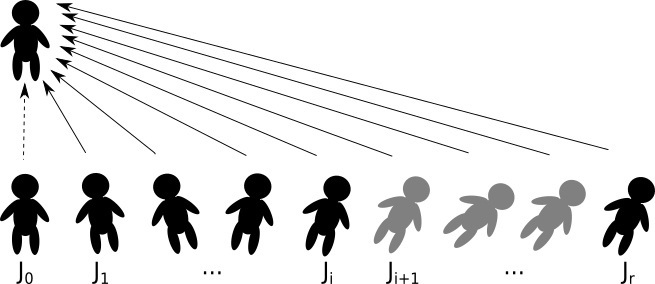
\includegraphics[width=.7\textwidth]{4/traditional-registration.png}
\label{fig:ch4:traditional-reg}
\caption{The traditional approach to volume registration in an rs-fMRI sequence consists of registering all volumes in the sequence to a single reference volume.}
\end{figure}

When performing image registration on a sequence of image volumes, one volume must be chosen as the reference volume for the entire sequence. All other volumes in the sequence are registered to this volume. An example of this process can be seen in Figure \ref{fig:ch4:traditional-reg}. In subsequent work, Friston et al. used the first volume in the rs-fMRI sequence as the universal reference image \cite{Friston1996}. Common choices for the reference volume include the volume with the least FD to all other volumes in the sequence, a volume produced by averaging all volumes in the sequence, or the first volume in the sequence \cite{Friston1996} \cite{Liao2005}. In our implementation, we chose to use the first volume in the sequence as the reference volume.

One drawback to this traditional approach to volume registration is that it only minimizes the differences between all the image volumes in the sequence and the reference volume. The key word here is minimizes: minimizing differences between image volumes does not mean that there are no differences between the image volumes. Image registration is an optimization problem, and its goal is to find the overlap between a pair of volumes with as few differences as possible either within a defined time period or until the optimization cost does not change above a certain tolerance for a certain amount of time. These practical constraints on optimization problems mean that there may still be differences between other pairs of image volumes in the sequence that do not include the reference volume. 

%Variations on Friston et al.'s framework have been developed over the last two decades. Liao et al. suggested that a rs-fMRI sequence could be viewed as a hidden Markov model, and reflected this idea in their suggested registration framework \cite{Liao2016}. They still use the first volume in the image sequence as the reference volume. Their framework uses the transformation of the previous volume to the reference volume to initialize the transformation for the current volume and the reference volume. 

%The success of volume registration in an rs-fMRI sequence is defined by the framewise differences between temporally neighboring image volumes.  During the registration process, the three translation and three rotation parameters can be used to calculate the displacement between a pair of images, which is often referred to as the framewise displacement (FD). Three groups have proposed slightly different methods for calculating the FD: Power et al., Jenkinson et al., and DOsenbach et al. \cite{Power2012} \cite{Jenkinson2002} \cite{Dosenbach2017}. All three FD calculations produce correlated metrics: the FD metric proposed by Power et al. produces measurements approximately twice as large as the metric proposed by Jenkinson et al., and Dosenbach et al. reported a high correlation between their FD and Power's FD \cite{Yan2013a} \cite{Dosenbach2017}.

%The FD metric only measures the positional effects of motion, not the variations in signal in individual voxels caused by motion. Changes in signal between volumes can be measured using the temporal derivative of the variance in the BOLD signal intensity (DVARS) between neighboring volumes \cite{Power2012} \cite{Smyser2015}. DVARs is an effective measure of the spin gradient effects of motion because it measures the change in BOLD signal intensity, which is highly related to motion-induced spin gradient changes. 

\subsection{Directed Acyclic Graph Based Registration}

In our proposed framework, we wish to account for the spatiotemporal relationships between temporally neighboring volumes in the sequence. To accomplish this goal, we start by viewing the rs-fMRI sequence as a directed acyclic graph (DAG). A DAG consists of a set of nodes and edges. Each edge has a direction associated with it and connects a pair of nodes. Since a DAG contains no cycles, there is no possible path back to a node once it has been traversed. 

\begin{figure}
\centering
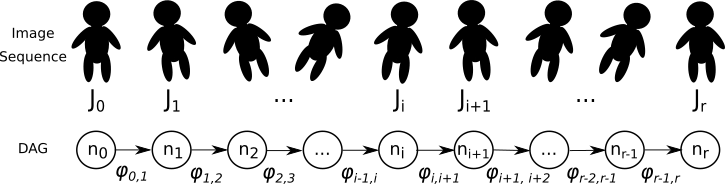
\includegraphics[width=.7\textwidth]{4/dag-chain.png}
\caption{A rs-fMRI can be viewed as a directed acyclic graph where each volume is a node and the edges connect from each volume $i$ to the following volume $i+1$.}
\label{ch4:fig:dag-chain}
\end{figure}

In the case of a rs-fMRI, each volume can be considered a node. The relationship between each pair of temporally neighboring volumes is represented as a directed edge connecting the node for the first volume to the node for the next volume. The acyclic nature of the DAG means that once a patient was in a specific position, he will never return to that exact same position with the exact same neurons firing. The position of the subject and his brain activity as measured by the BOLD signal may be similar in subsequent image volumes, but it will never be precisely the same. The perspectives of an rs-fMRI sequence as a set of images and of the sequence as a DAG can be seen in Figure \ref{ch4:fig:dag-chain}.

The cost of transitioning from one node to the next in our DAG has a parallel representation to the combination of the positional transformation needed to align volume $i$ to volume $i+1$ and the signal change between the volumes. This representation can be written as 

\begin{equation}
J_{i+1} = \phi_{i,i+1} J_i + \delta s_{i,i+1} + \epsilon
\end{equation}

\noindent{where $J_i$ and $J_{i+1}$ are volumes $i$ and $i+1$, $\phi_{i,i+1}$ is a matrix of transformation parameters that must be applied to $J_i$ to achieve the patient’s position in $J_{i+1}$, $\delta s_{i,i+1}$ is the natural change in BOLD signal, and $\epsilon$ is the change in BOLD signal due to motion. Currently, there is no way to estimate the natural change in BOLD signal and the change in BOLD signal due to motion without incorporating additional information about the MRI scanner and the patient that is not included in a rs-fMRI. We simplify our representation of the relationship between two volumes to}

\begin{equation}
J_{i+1} = \phi_{i,i+1} J_i + \epsilon^*
\end{equation}

\noindent{where $\epsilon^*$ is the change in the BOLD signal that cannot be accounted for after aligning the patient’s position in the two volumes. Here, we use the notation $\epsilon^*$ to represent the generic error change in BOLD signal across any pair of volumes.}

After aligning two volumes $i$ and $i+1$, we will then align volumes $i+1$ and $i+2$:

\begin{equation}
\begin{split}
J_{i+2} &= \phi_{i+1,i+2} J_{i+1} + \epsilon^* \\
&= \phi_{i+1,i+2} (\phi_{i,i+1} J_i + \epsilon^*) +\epsilon^*\\
&= \phi_{i+1,i+2} \phi_{i,i+1} J_i + \epsilon^{*'}\\
\end{split}
\end{equation}

Traditional volume registration assumes that 

\begin{equation}
\phi_{i,i+2} = \phi_{i+1,i+2} \phi_{i,i+1}
\end{equation}

\begin{figure}
\centering
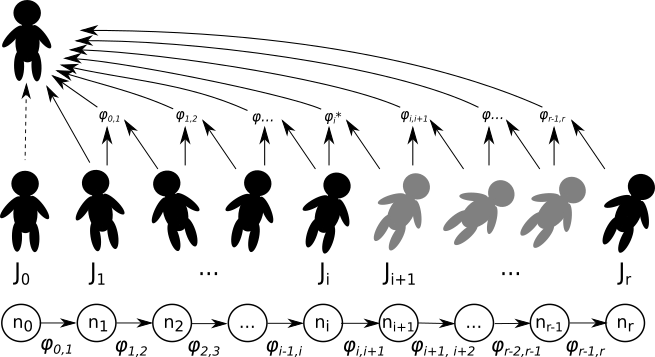
\includegraphics[width=.7\textwidth]{4/dag-registration.png}
\label{ch4:fig:dag-reg}
\caption{The traditional approach to volume registration in an rs-fMRI sequence consists of registering all volumes in the sequence to a single reference volume.}
\end{figure}

\noindent{and calculates $\phi_{i,i+2}$ directly. We argue that this assumption is not true in all cases. Rather than directly calculate $\phi_{0,i}$ and use it to align volume $i$ to the reference volume as the traditional method does, we calculate each component $\phi$ that is a factor of $\phi_{0,i}$. Each component $\phi_{i,i+1}$ is combined with the preceding $\phi_{0,i}$s to recursively align volume $i+1$ to the reference volume without making the large and often inaccurate transformations required by directly calculating $\phi_{0,i+1}$.} This process is outlined in Figure \ref{ch4:fig:dag-reg}.

\subsection{Motion Correction Pipeline}

After performing both volume registration techniques independently on all images, both registered versions of the images will undergo motion correction. Many pipelines exist for correcting motion in rs-fMRIs. We choose to use a method which uses independent component analysis. 

\section{Motion Metrics}

Power et al. thresholds

%The global volume registration techniques were applied to all 17 resting-state BOLD MR images. After the registrations, each subject had three sequences associated with it: the original sequence, the sequence registered using the traditional framework, and the sequence registered using the DAG-based framework. The globally registered images were compared to each other in terms of correlation ratios between all volumes in the sequence as well as FD and DVARS between temporally neighboring volumes. 

Correlation ratio matrix

%The correlation ratio is an asymmetrical, spatially informed measure of the overlap between images where volumes with better alignment will have lower correlation ratios \cite{Roche1998}. For each sequence, we used FLIRT (FMRIB’s Linear Image Registration Tool) to calculate the correlation ratio between each possible pair of volumes in the sequence \cite{Jenkinson2001} \cite{Jenkinson2002}. We then used the average and standard deviation of the correlation ratio distribution of each image to compare the images. We also calculated the FD and DVARS metrics defined by Power et al. using the FSLMotionOutliers tool \cite{Power2012}. These metrics were calculated for each image and were used for evaluation of the efficacy of the registration frameworks.

Dice coefficients?

\section{Motion Patterns} 

We suggest that the ways that patients move are specific to certain patient groups. For example, fetal patients live suspended in amneotic fluid and as such are subject to different physical constraints than patients in other age groups. Neonatal patients are often scanned using a ``feed and bundle'' protocol, which often results in them sleeping through the scan. However, neonatal patients sometimes wake up during the scan. The way a baby woken up from a nap moves is different from how a fidgety preadolescent moves, though the terminology to define how these movement patterns differ is somewhat lacking. 

There is also a chance that patients within the same age group move differently possibly due to their cognitive state. Preadolescents who have ADHD likely become bored and fidgety in the MR scanner at different rates then their non-ADHD counterparts. Adults suffering from dementia may have more difficulty remaining still for the duration of a scan than adults with similar demographics and no dementia.

We have several goals for this portion of our work. The first is to identify features of the rs-fMRIs that are informative about patient movement during a scan. We will initially use the metrics described in the previous section, but may experiment with other metrics from the biomedical imaging and computer vision domains.

Our second goal is to group patients based on features extracted from their original images, their registered images, and their motion corrected images. Additional behavioral, clinical, and demographic data will also be used. We will use machine learning and statistical analysis techniques to identify relationships between different features or subsets of features. 

% If the relationships between different types of patient motion and behavioral, clinical, and demographic data are sufficiently strong, we will train a machine learning model to identify a patient's output variable based on his image features.

\section{Statistical Analyses}

\section{Implementation: Tools and Libraries}

The registration frameworks described in this section were implemented in Python using the nipype (Neuroimaging in Python Pipelines and Interfaces) library \cite{Gorgolewski2011}. Affine volume registration was performed using ANTs (Advanced Normalization Tools) \cite{Avants2014}. The metric used to estimate the dissimilarity between the pairs of volumes being registered was cross-correlation with a local window size of 5 voxels. 

Cite FSL, etc. here

